\documentclass[12pt, a4paper]{article}

\usepackage[T2A]{fontenc}
\usepackage[utf8]{inputenc}
\usepackage[english,russian]{babel}
\usepackage[left = 1.5 cm, right = 1.5 cm, top = 2cm, bottom = 2 cm, bindingoffset = 0 cm]{geometry}
\usepackage{amsmath,amsfonts,amssymb,amsthm,mathtools}
\usepackage{wasysym}
\usepackage{float}

\usepackage{tikz}

\usepackage{graphicx}
\graphicspath{{pictures/}}
\DeclareGraphicsExtensions{.pdf,.png,.jpg}

\usepackage{alltt}

\begin{document}
\begin{titlepage}
\newpage

\begin{center}
Министерство образования и науки Российской Федерации \\
Федеральное государственное автономное образовательное
учреждение высшего образования \\
Национальный исследовательский Нижегородский государственный
университет им. Н.И. Лобачевского \\
Институт информационных технологий, математики и механики \\
\end{center}

\vspace{12em}

\begin{center}
\textsc{\textbf{Отчёт по лабораторной работе}}\\
\textsc{\textbf{Численные методы исследования динамических систем с помощью пакета MatLab}}
\end{center}

\vspace{14em}



\newbox{\lbox}
\savebox{\lbox}{\hbox{Барабаш Н. В.}}
\newlength{\maxl}
\setlength{\maxl}{\wd\lbox}
\hfill\parbox{11cm}{
\hspace*{5cm}\hspace*{-2cm} \textbf{Выполнил:} студент группы 381803-1 \\
\hspace*{5cm}\hspace*{-2cm} Петров Павел \\
\hspace*{5cm}\hspace*{-2cm} \textbf{Проверил:} научный сотрудник \\
\hspace*{5cm}\hspace*{-2cm} лаборатории динамического хаоса \\
\hspace*{5cm}\hspace*{-2cm} кафедры ТУиДС \\
\hspace*{5cm}\hspace*{-2cm} Казаков А. О. \\
\\
}


\vspace{\fill}
\vspace{\fill}

\begin{center}
Нижний Новгород \\2021
\end{center}

\end{titlepage}
\section{Аттрактор Лоренца}
Рассмотрим систему Лоренца и построим для неё бифуркационную диаграмму.
\begin{equation*}
	\begin{cases}
		\dot x = \sigma (y - x) \\
		\dot y = x(r - z) - y \\
		\dot z = xy - bz
	\end{cases}
\end{equation*}
$\sigma, \; r, \; b$ - положительные параметры.

Построим кривую $l_1$.
\newline
В Starter выберем момент времени $t=0$ и точку $(x,y,z) = (0.001, 0, 0)$. В Integrator выставим параметр interval в 2,5. Параметры - $(\sigma, r, b) = (10, 14, \frac{2}{3})$. Построим кривую. Далее выберем начальную точку как состояние равновесия: $\textbf{Type|Initial Point|Equilibrium}$, а кривую - $\textbf{Type|Curve|ConnectionSaddle}$. Нажмём $\textbf{Compute|Forward}$ и затем в Data Browser выберем HTHom Select Connection. После этого выбираем в Starter параметры (r, SParam1, eps1) и зануляем параметр SParam1. В Data Browser выбираем HTHom SParam1 equal to zero. Теперь выберем параметры (r, eps1, T) и будем занулять eps1. Выбираем в Data Browser HTHom eps1 small enough, а в initializer - Homoclinic to Saddle. Выбираем параметры (s, r, T) и начинаем строить кривую $l_1$.
\begin{figure}[H]
	\center{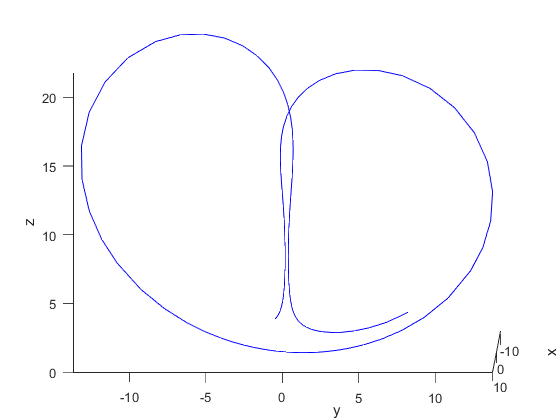
\includegraphics[scale=0.7]{LorenzLL1}}
	\caption{Выбор Connection Saddle}
\end{figure}
\begin{figure}[H]
	\center{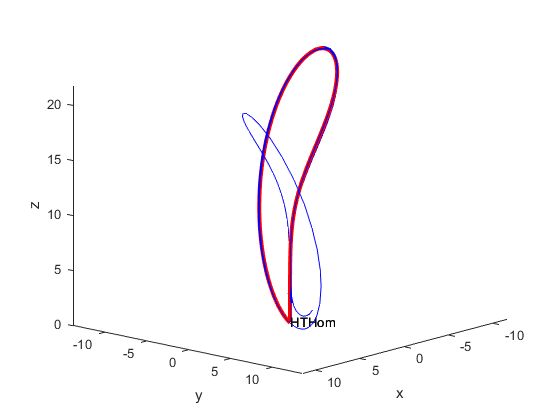
\includegraphics[scale=0.7]{LorenzLL12}}
	\caption{Зануляем SParam1 и eps1}
\end{figure}
\begin{figure}[H]
	\center{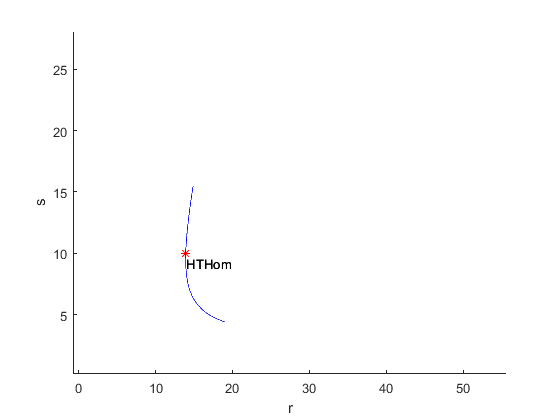
\includegraphics[scale=0.7]{LorenzLL13}}
	\caption{Кривая бифуркации гомоклинической восьмёрки бабочки}
\end{figure}
Построим кривую $l_3$ бифуркации Андронова-Хопфа.
\newline
В Starter выберем момент времени $t=0$ и точку $(x,y,z) = (0.001, 0, 0)$. Параметры - $(\sigma, r, b) = (10, 2, \frac{2}{3})$ Найдём состояние равновесия и затем выберем эту точку как состояние равновесия: $\textbf{Type|Initial Point|Equilibrium}$. Протянем её по параметру $r$, пока не найдём точку Hopf. Выберем её в Initializer, выберем пункт Hopf (init\_H\_H), затем, протянув по двум параметрам $(\sigma, r)$, получим кривую $l_3$.
\begin{figure}[H]
	\center{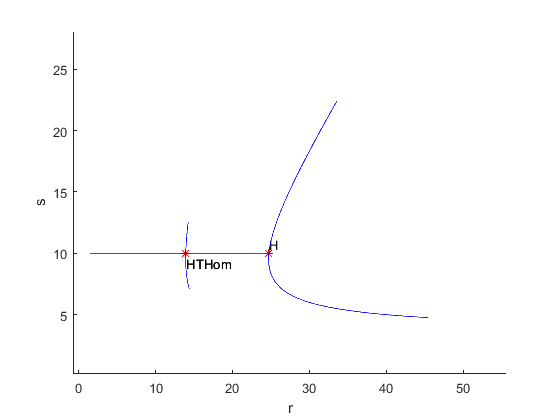
\includegraphics[scale=0.8]{lorenzl2}}
	\caption{Кривая бифуркации Андронова-Хопфа}
\end{figure}
Построим кривую симметричной бифуркации вилки.
\newline
Для этого при тех же параметрах и начальной точке находим состояние равновесия, затем протягиваем его по r в сторону уменьшения, пока не наткнёмся на Branch Point. Выберем эту точку в Data Browser, а в Initializer выберем Equilibrium (BP). Далее протягиваем бифуркационную кривую по параметру $\sigma$.
\begin{figure}[H]
	\center{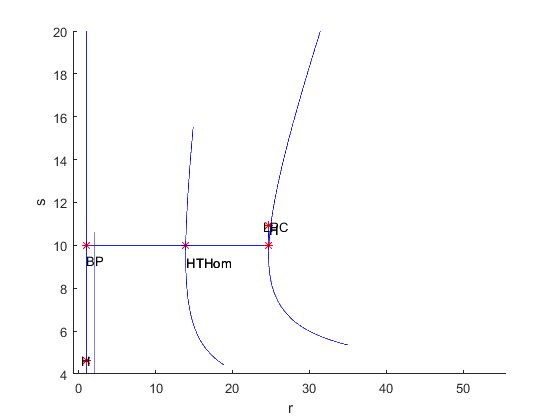
\includegraphics[scale=0.8]{LorenzLL14}}
	\caption{Кривая бифуркации вилка}
\end{figure}

\section{Система Шимицу-Мориока}
Рассмотрим систему:
\begin{equation*}
	\begin{cases}
		x' = y \\
		y' = x - ay - xz \\
		z' = -bz + x^2
	\end{cases}
\end{equation*}
$a > 0$ и $b > 0$ - параметры.
\newline
Протянем бифуркацию Андронова-Хопфа. Для этого выберем точку в окрестности нуля и параметры $(a, b) = (1.5; 0.38)$. Находим состояние равновесия, выбираем найденную точку и протягиваем её по параметру $a$ как $equilibrium$. Находим точку $Hopf$ и протягиваем её по двум параметрам.
\begin{figure}[H]
	\center{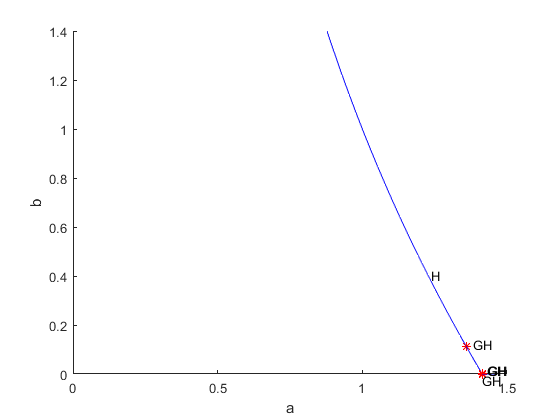
\includegraphics[scale=0.8]{SMHopf}}
	\caption{Кривая бифуркации Андронова-Хопфа}
\end{figure}
Построим кривую бифуркации $HB$. Выберем точку в окрестности нуля и параметры $(a, b) = (1.225; 0.38)$. Простроим кривую, выбрав параметр $interval$ равным 25. Далее выберем начальную точку как состояние равновесия: $\textbf{Type|Initial Point|Equilibrium}$, а кривую - $\textbf{Type|Curve|ConnectionSaddle}$. Нажмём $\textbf{Compute|Forward}$ и затем в Data Browser выберем HTHom Select Connection. После этого выбираем в Starter параметры (a, SParam1, eps1) и зануляем параметр SParam1. В Data Browser выбираем HTHom SParam1 equal to zero. Теперь выберем параметры (a, eps1, T) и будем занулять eps1. Выбираем в Data Browser HTHom eps1 small enough, а в initializer - Homoclinic to Saddle. Выбираем параметры (a, b, T) и начинаем строить кривую бифуркации $HB$.

\begin{figure}[H]
	\center{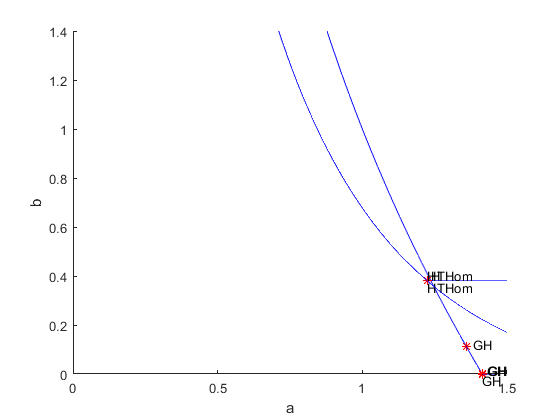
\includegraphics[scale=0.8]{SMHB}}
	\caption{Кривая бифуркации HB}
\end{figure}

Найдём нейтральное седло путём выбора нулевой точки как $Equilibrium$. Протянем её по параметру $b$. Наткнёмся на точку $Neutral-Saddle$ $equilibrium$, выберем её и протянем по двум параметрам.

\begin{figure}[H]
	\center{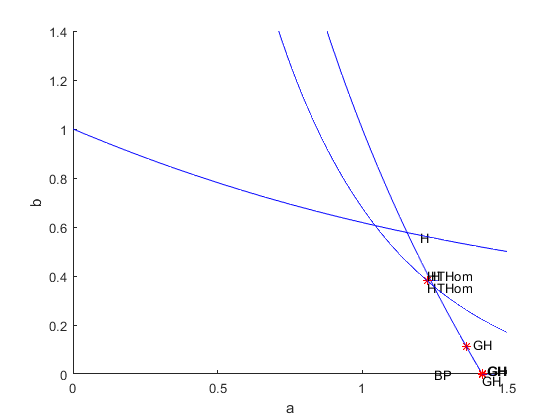
\includegraphics[scale=0.8]{SMNS}}
	\caption{Кривая нейтрального седла}
\end{figure}

Вытянем кривую седло-узловой бифуркации из точки $Generalized$ $Hopf$. Выберем её и выберем тип кривой $limit$ $point$ $of$ $cycles$.

\begin{figure}[H]
	\center{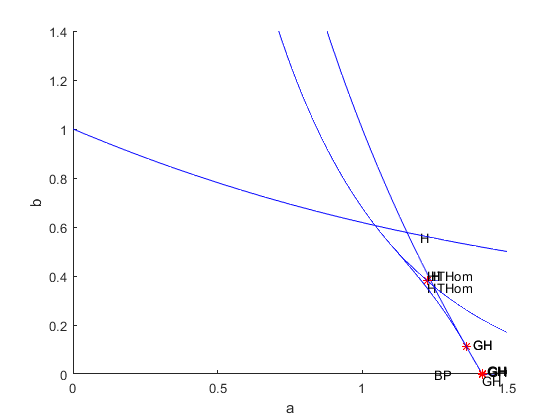
\includegraphics[scale=0.8]{SMSaddleNode}}
	\caption{Кривая седло-узловой бифуркации}
\end{figure}

Выберем точку в окрестности нуля и параметры $(a, b) = (0.62, 0.4)$. Проделаем те же действия, что и с кривой $HB$.

\begin{figure}[H]
	\center{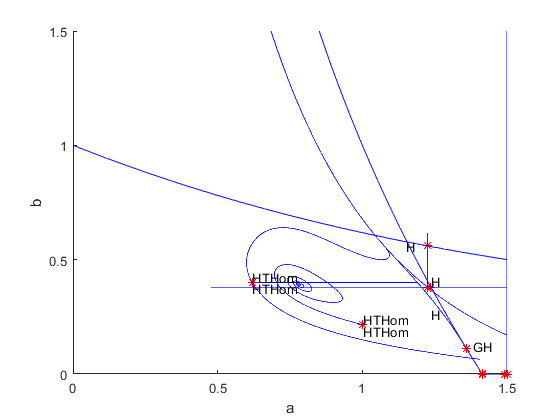
\includegraphics[scale=0.8]{ShimitsuMarioca1}}
	\caption{Кривая HB-2}
\end{figure}

\section{Система Рёсслера}

Рассмотрим систему вида:
\begin{equation*}
	\begin{cases}
		\dot x = - y - z \\
		\dot y = x + a  y \\
		\dot z = b  x + z  (x - c)
	\end{cases}
\end{equation*}

Приравняв правые части нулю, получим систему:
\begin{equation*}
	\begin{cases}
		y = -z \\
		x = -ay = az \\
		abz + z(az - c) = 0
	\end{cases}
\end{equation*}

Из которой легко извлечь, что состояниями равновесия являются $O_1 = (0, 0, 0)$ и $O_2 = (c - ab; \frac{ab - c}{a}; \frac{c - ab}{a})$.

Построим области устойчивости, вычислив характеристический многочлен линеаризованных в окрестности данных состояний равновесия систем и получив условия на коэффициенты с помощью следствия из критерия Рауса-Гурвица.

Для $O_1$ характеристический многочлен имеет вид:
$ \lambda^3 - (a - c)\lambda^2 - (ac - 1.3)\lambda - 0.3a + c = 0 $
и область устойчивости:
\begin{equation*}
	\begin{cases}
		a - c < 0 \\
		ac - 1.3 < 0 \\
		c - 0.3 a > 0 \\
		(a - c)(ac - 1.3) > c - 0.3 a
	\end{cases}
\end{equation*}

Для $O_2$ характеристический многочлен имеет вид:
$ \lambda^3 + 0.7 a \lambda^2 + (0.3a^2 - \frac{c}{a} - 1)\lambda - 0.3a + c = 0 $
и область устойчивости:
\begin{equation*}
	\begin{cases}
		a > 0 \\
		0.3a^2 - \frac{c}{a} - 1 > 0 \\
		c - 0.3 a > 0 \\
		0.7a(0.3a^2 - \frac{c}{a} - 1) > c - 0.3 a
	\end{cases}
\end{equation*}

\begin{figure}[H]
	\center{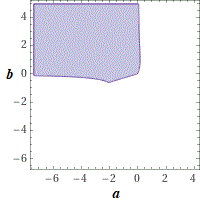
\includegraphics[scale=0.8]{ZeroEQSTRoessler}}
	\caption{Область устойчивости нулевого состояния равновесия}
\end{figure}

\begin{figure}[H]
	\center{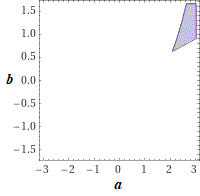
\includegraphics[scale=0.8]{NonZeroEQSTRoessler}}
	\caption{Область устойчивость ненулевого состояния равновесия}
\end{figure}

Найдём бифуркационные кривые, отвечающие бифуркации Андронова-Хопфа. Для этого выберем точку в окрестности нуля, подберём параметры так, чтобы ноль был устойчив. Найдём устойчивое состояние равновесия и с помощью протягивания параметра $a$ будем искать точки бифуркаций. Далее выбираем эти точки и протягиваем их уже по двум параметрам $a$ и $c$.

\begin{figure}[H]
	\center{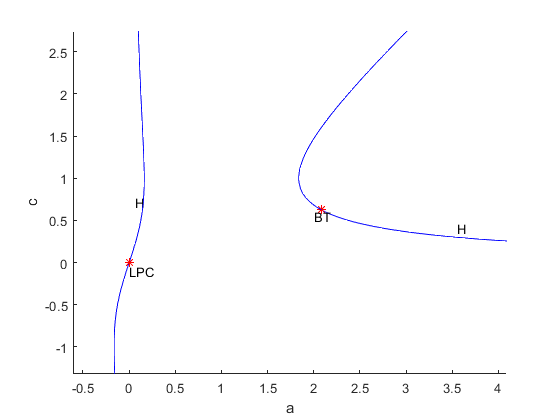
\includegraphics[scale=0.8]{RosslerHopf}}
	\caption{Кривые бифуркаций Андронова-Хопфа}
\end{figure}

Проследим за эволюцией аттрактора в системе. Для этого зафиксируем параметры $b = 0.3$ и $c = 4.9$, изменять будем $a$.

\begin{figure}[H]
	\center{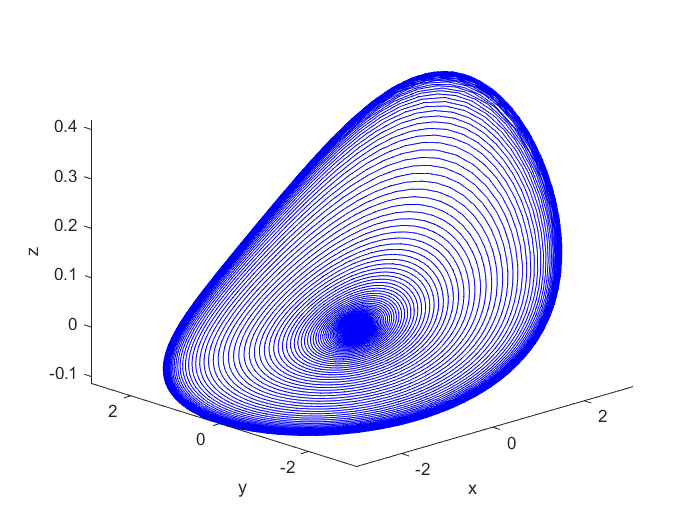
\includegraphics[scale=0.8]{RosAtr1}}
	\caption{$a = 0.08$}
\end{figure}

\begin{figure}[H]
	\center{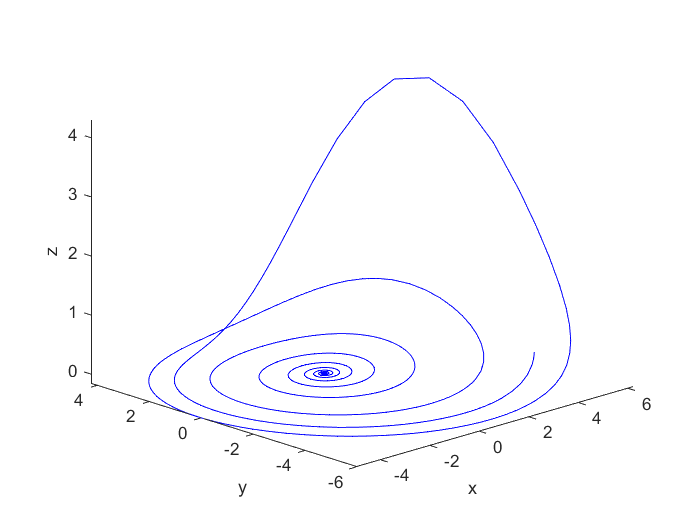
\includegraphics[scale=0.8]{RosAtr2}}
	\caption{$a = 0.25$}
\end{figure}

\begin{figure}[H]
	\center{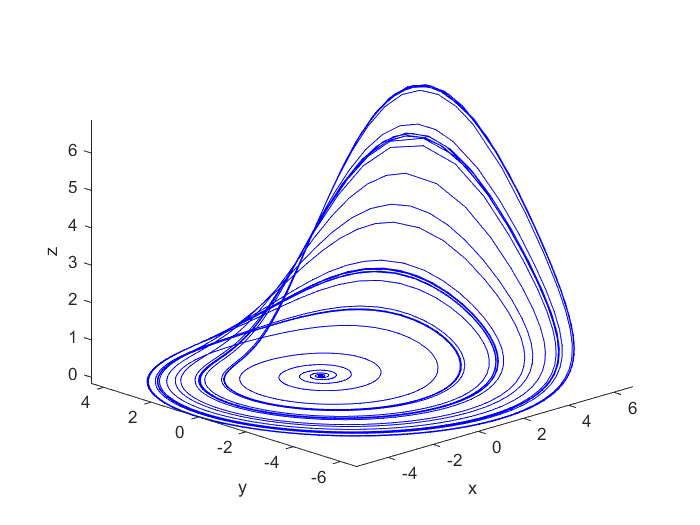
\includegraphics[scale=0.8]{RosAtr3}}
	\caption{$a = 0.275$}
\end{figure}

\begin{figure}[H]
	\center{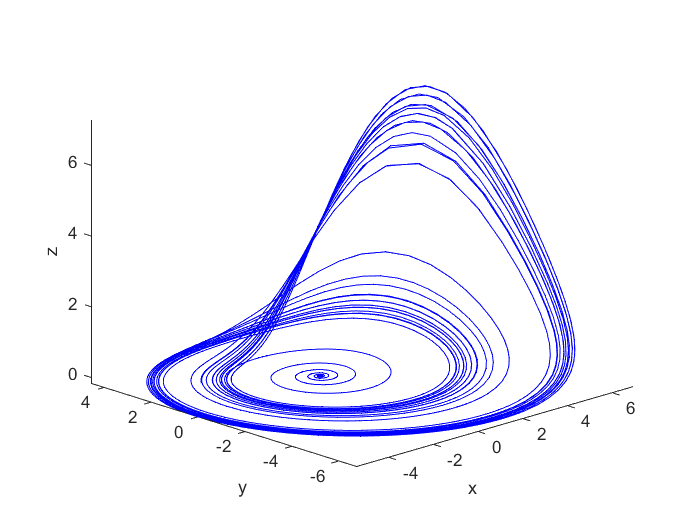
\includegraphics[scale=0.8]{RosAtr4}}
	\caption{$a = 0.28$}
\end{figure}

\begin{figure}[H]
	\center{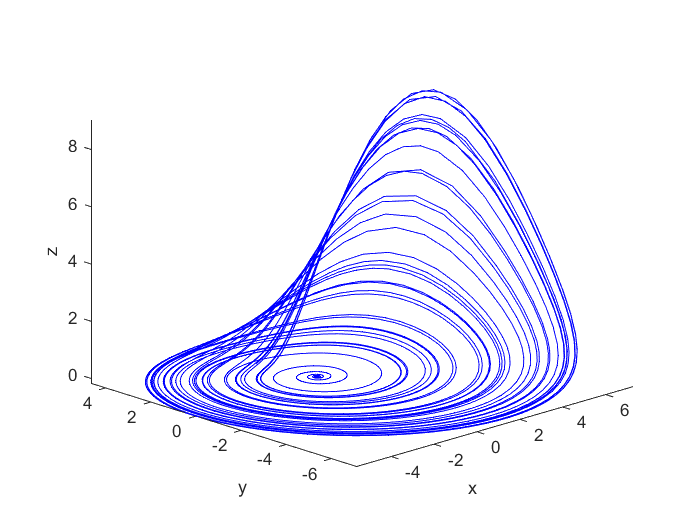
\includegraphics[scale=0.8]{RosAtr5}}
	\caption{$a = 0.3$}
\end{figure}

\begin{figure}[H]
	\center{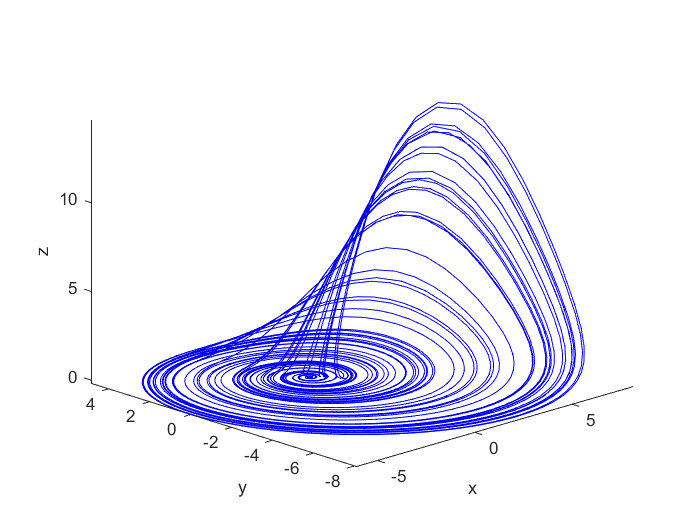
\includegraphics[scale=0.8]{RosAtr6}}
	\caption{$a = 0.35$}
\end{figure}

Найдём в Матконте кривые гомоклинических бифуркаций h1 и h2. Для кривой h1 выберем параметры $(a, b, c) = (0.35, 0.3, 4.88573)$, а для h2 - $(a, b, c) = (0.47, 0.3, 4)$, параметр $interval = 5$. И повторим ту же процедуру, что была проделана для отыскания кривой гомоклинической бифуркации в системе Лоренца.

\begin{figure}[H]
	\center{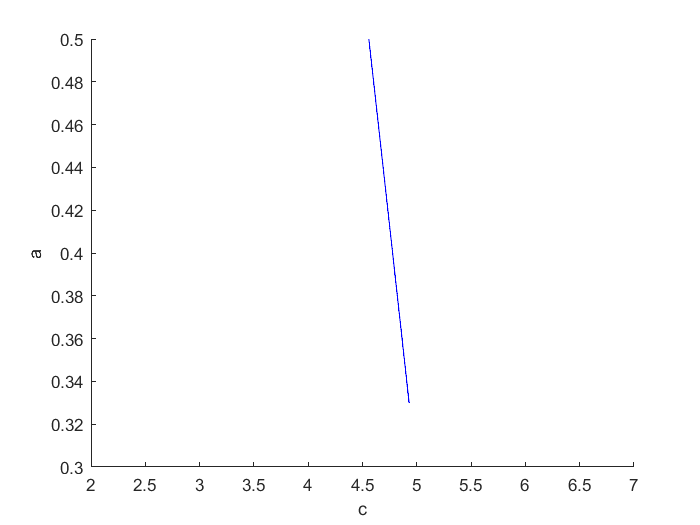
\includegraphics[scale=0.8]{RosslerH1}}
	\caption{Кривая h1}
\end{figure}

\begin{figure}[H]
	\center{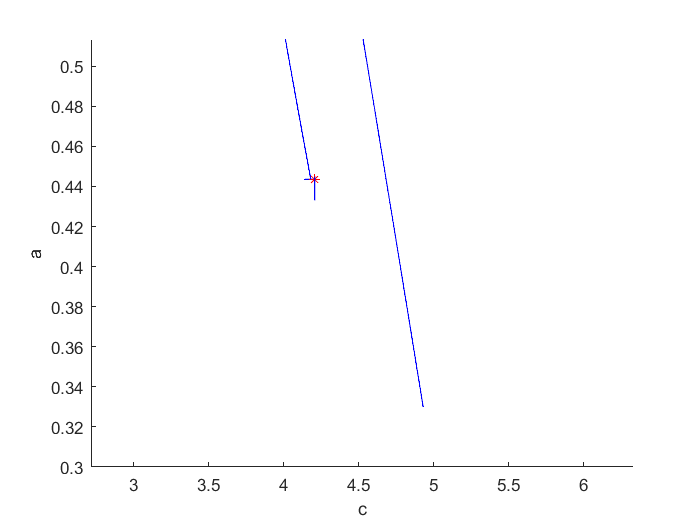
\includegraphics[scale=0.8]{RosslerH2}}
	\caption{Кривая h2}
\end{figure}

Построим окно устойчивости $S_1$. Для этого при параметрах $(a, b, c) = (0.3 0.3 0.73)$ ищем цикл. Сначала строим траекторию при $intervals = 80$, затем выбираем конечную точку на траектории и считаем от неё при $intervals = 20$. После просчёта траектории выбираем её как $limit$ $cycle$ и поочерёдно протягиваем по параметрам $(a, T)$, $(c, T)$, $(a, c)$, чтобы отыскать нужные нам точки, например, Limit point of cycle или Period Doubling. Выбирая их и протягивая по параметрам $(a, c)$, получаем нужные нам кривые.

\begin{figure}[H]
	\center{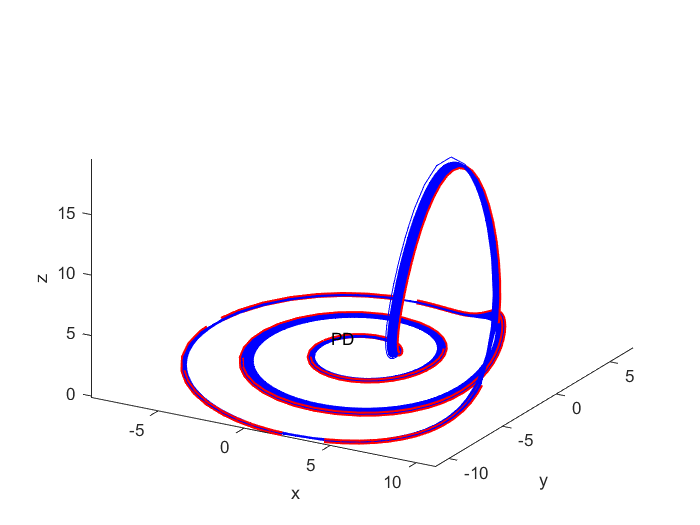
\includegraphics[scale=0.6]{cycle}}
	\caption{Процесс отыскания нужных нам кривых}
\end{figure}

\begin{figure}[H]
	\center{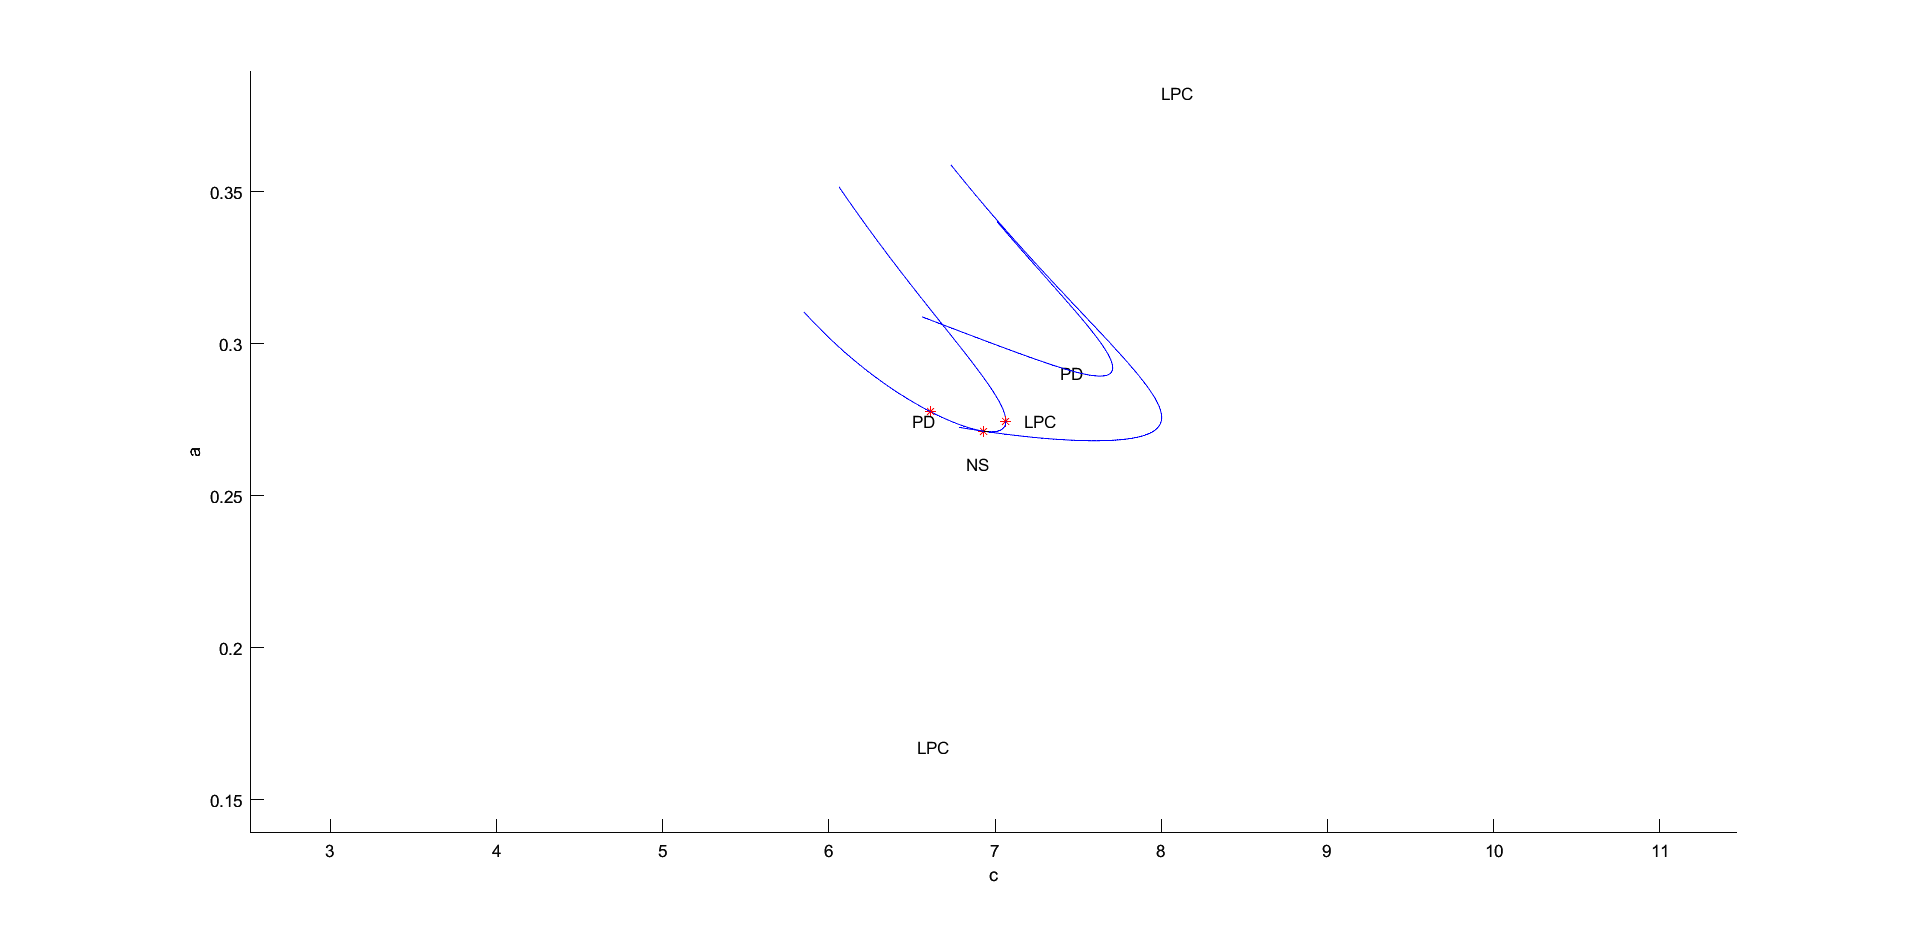
\includegraphics[scale=0.25]{RosS1}}
	\caption{Окно устойчивости S1}
\end{figure}

\begin{figure}[H]
	\center{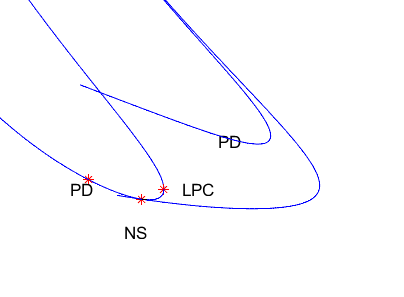
\includegraphics[scale=0.8]{RosS1PLUS}}
	\caption{Окно устойчивости S1 в масштабе}
\end{figure}

\end{document}